\section{Introduction}
\label{sec:introdcution}

%%%%%%%%%%%%%%%%%%%%%%%%%%%%%%%%%%%%%%%%%

Executing tasks requiring complex dynamic motions, such as running, jumping, or navigating uneven terrain, demands careful consideration of the dynamic properties of the low-level joint actuation. Specifically, implementing torque-controlled dynamic motion in bipedal robots using electric actuators is particularly complex, especially in the absence of joint torque sensors. Achieving precise torque control necessitates developing and implementing control algorithms that incorporate accurate dynamic modeling, as well as the identification of motor characteristics and harmonic drive properties. Many humanoid robots, such as ergoCub, iCub3, PAL Robotics' REEM-C, and RoK-3, utilize a combination of motors and high-reduction gears, such as Harmonic Drives, to generate the substantial torques needed for their joints given the robot's weight~\cite{dafarra2024icub3,han2022slope,ossadnik2018adaptive,han2023implementing}. However, high-reduction gears pose significant challenges, including high friction and low backdrivability. This high friction can introduce considerable delays between torque input and output, complicating torque control, especially when rapid responses to dynamically changing torque are required. Furthermore, high friction leads to energy losses, increased wear and tear, and reduced efficiency, ultimately degrading the precision and responsiveness of joint movements. Addressing these challenges requires sophisticated friction models and compensation strategies~\cite{marques2016survey}.

Friction identification can be performed using model-based or learning-based approaches. Model-based approaches, such as Coulomb, viscous, LuGre, Dahl, Leuven, and generalized Maxwell-slip models, are typically categorized into static and dynamic friction models~\cite{awrejcewicz2005analysis}. Static models have limitations in capturing the full spectrum of frictional phenomena and often yield less accurate results than dynamic models~\cite{iurian2005identification}. Moreover, many existing static friction models struggle with discontinuity when transitioning from the pre-sliding to the sliding regime~\cite{olejnik2013application, jin2019joint}.
% Static models have limitations in capturing the full spectrum of frictional phenomena and often yield less accurate results than dynamic models \cite{iurian2005identification}. Moreover, many existing static friction models struggle with discontinuity when transitioning from the pre-sliding to the sliding regime~\cite{olejnik2013application, jin2019joint}.
\looseness=-1
\begin{figure}[t]
\centering
\begin{subfigure}{.49\columnwidth}
  \includegraphics[width=\textwidth]{figures/ergocub_crain.png}
  \label{fig:ergocub_front}
\end{subfigure}%
\hspace{\fill} % Add horizontal space between subfigures
\begin{subfigure}{.49\columnwidth}
  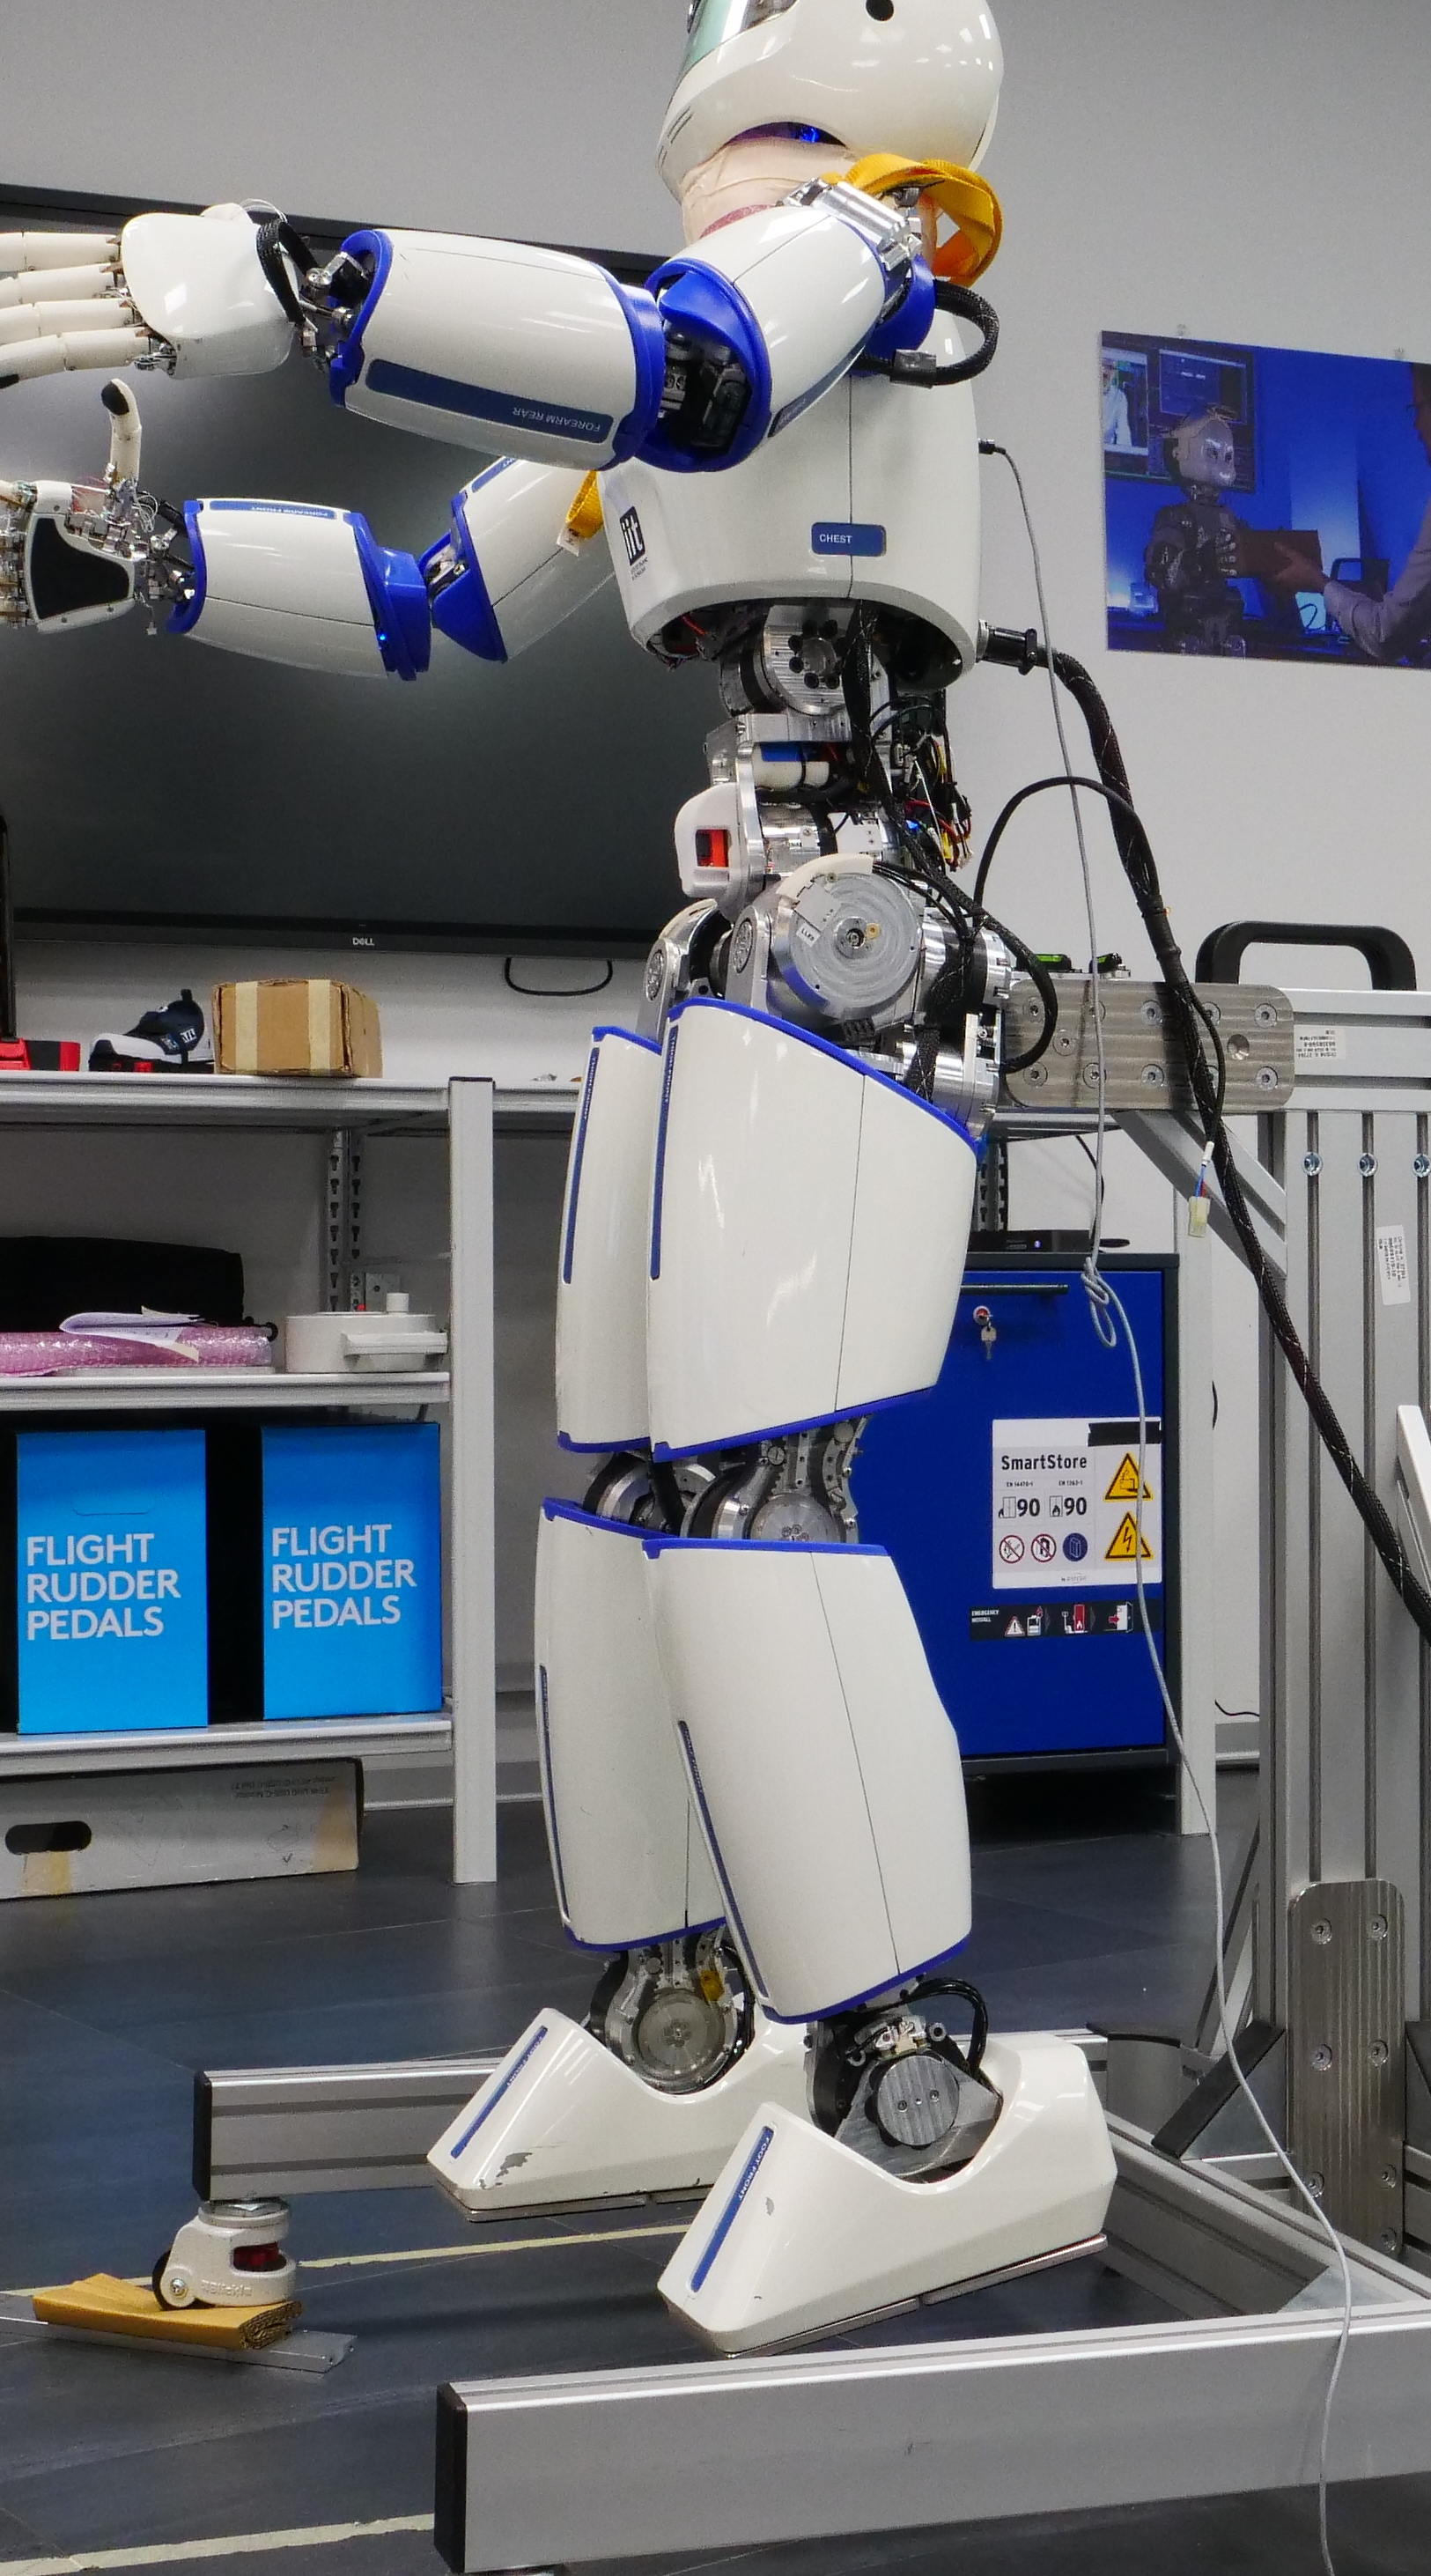
\includegraphics[width=\textwidth]{figures/ergocub_pole.png}
  \label{fig:ergocub_lat}
\end{subfigure}
\vspace{-20pt}
\caption{The ergoCub humanoid robot.}
\label{fig:ergocub}
\vspace{-20pt}
\end{figure}
The Coulomb-viscous friction model is sufficient for depicting the frictional behavior within multi-body dynamic systems for many applications. For example, the Coulomb-viscous model can estimate and compensate for torque losses during the landing impact of a biped robot~\cite{nagamatsu2017distributed}. The model can be improved by integrating the Stribeck effect, achieving more accurate friction compensation~\cite{jin2019joint}. Nevertheless, traditional static and dynamic friction models typically rely on simplified assumptions and linear approximations, failing to capture the complex system dynamics. In the case of high-ratio harmonic drives, friction exhibits highly non-linear behavior and complex dependencies on various states and conditions, such as the variation of temperature or the presence of backlash, especially during direction changes or low-speed movements~\cite{wolf2018extending}.

% The Coulomb-Viscous friction model is sufficient for depicting the frictional behavior within multi-body dynamic systems for many applications. For example, the Coulomb-viscous model can estimate and compensate for torque losses during the landing impact of a biped robot \cite{nagamatsu2017distributed}. The model can be improved by integrating the Stribeck effect, achieving a more accurate friction compensation \cite{jin2019joint}. Nevertheless, traditional static and dynamic friction models typically rely on simplified assumptions and linear approximations, failing to capture complex system dynamics. In the case of high-ratio harmonic drives, friction exhibits highly non-linear behavior and complex dependencies on various states and conditions, such as the variation of temperature or the presence of backlash, especially during direction changes or low-speed movements~\cite{wolf2018extending}.
\looseness=-1

Models based on Neural Networks (NN) have advantages in modeling complex systems by learning directly from the data. Research on using NN to develop friction models for robot joints is limited, especially for humanoid robots equipped with electric motors and high-ratio harmonic drives. One approach uses a back-propagation NN, optimized by a genetic algorithm, to model static friction in a robot joint~\cite{tu2019modeling}. A second solution models rolling friction using Long Short-Term Memory (LSTM)~\cite{wang2023improved}. However, these approaches require large datasets to ensure diverse and representative training data. Moreover, LSTMs are more computationally intensive than simple feedforward NNs, making it harder to scale for multiple humanoid robot joints while maintaining real-time performance and a low computational load. To overcome these limitations a study identifies the planar frictional torque acting at the contact surface of a double torsion pendulum by adopting a Physics Informed Neural Network (PINN)~\cite{olejnik2023friction}. PINNs overcome problems of small datasets by informatively exploiting a priori knowledge of the non-linear system for constructing robust feedforward NNs. In the physics-informed modeling framework, training of the NN is facilitated by directly embedding the underlying governing physical laws as regularization terms in the cost function of the learning problem.\looseness=-1

Friction identification procedures often require specialized setups, as shown in~\cite{wang2023improved}, where data were collected from an emulated industrial machine axis. However, such setups are not always available, making this technique impractical in many scenarios. An alternative is to collect data directly from the robot, as demonstrated in~\cite{tu2019modeling}, which uses motor angular velocities and joint load torques as inputs for the NN. This method, however, fails when the joint load torque is unknown. When measuring the ground truth is not feasible, friction torque can be computed through dynamic modeling, as in~\cite{olejnik2023friction}. Yet, this approach, tested on a double torsion pendulum, is unsuitable for our problem for two reasons. First, our system incorporates harmonic drives, while the system in~\cite{olejnik2023friction} does not. Second, their method requires two NNs to predict friction torque and angular rotation, which adds computational complexity, making it impractical for humanoid robots with many degrees of freedom.
\looseness=-1

This paper contributes to developing a robust and scalable friction identification method based on Physics-Informed Neural Networks (PINN). The PINN model inputs the history of the position error between joint and motor positions, and joint velocities. This method is specifically tailored for robots with electric motors and high-ratio harmonic drives. Our approach does not require dedicated setups for data acquisition. The pipeline is versatile and applicable to all joints of a humanoid robot, making it neither joint nor robot-dependent. The chosen identification model (PINN) is computationally efficient, enabling scalability to all joints of a humanoid robot while maintaining real-time performance.\looseness=-1

Additionally, we test the PINN model's effectiveness by comparing it with classical static friction models, specifically Coulomb-viscous and Stribeck-Coulomb-viscous. The identification and testing processes are conducted on the humanoid robot ergoCub. The data acquisition procedure involves the accurate selection of exciting trajectories and thorough data processing. We incorporate the estimated friction models into a real-time friction compensation system integrated with a joint torque control architecture~\cite{sorrentino2024ukf}. We demonstrate that the PINN model reduces energy losses to achieve the same high-level tracking performance as the other models.\looseness=-1

The paper is organized as follows. Sec.~\ref{sec:background} introduces the notation and recalls some concepts of floating-base systems, harmonic drive model, an overview of static friction models, and the Physics Informed Neural Network model. Sec.~\ref{sec:methods} details the friction models identification procedure. Sec.~\ref{sec:results} presents the validation results on two diffent joints of the humanoid robot ergoCub. Sec.~\ref{sec:conclusions} concludes the paper.\looseness=-1